\chapter{Device 1: prototype for spatio-angular illumination}
\begin{summary}
   - Im vorhergehende Kapitel haben wir das dem spatio-angularen
     Mikroskop zugrundliegende Konzept dargestellt. Hier gehen wir auf
     zusaetzliche Details ein, die fuer die praktische Implementierung
     wichtig sind. Unter anderem die Eigenschaften der beiden
     verwendeten Displays, elektronische Synchronisation der
     verschiedenen Komponenten und einem Algorithmus, um das             % /Hier mehr spezifische Probleme/
     Koordinatensystem der Kamerapixel und der Pixel des focal plane
     SLM ineinander zu transformieren.

   - Das pupil plane SLM wurde durch unseren Partner Fraunhofer IPMS
     waehrend des Projekts neu entwickelt.  Daher widmen wir uns diesem   % /MMA kommt spaeter extra/
     Subsystem im Kapitel (FIXME) naeher.
\end{summary}
\section{Beschreibung der optischen Komponenten}
 - Bisher haben wir den Strahlengang nur fuer Transmissionsdisplays
   gezeigt (in fig:memi-simple). Solche SLM haben in Praxis aber nur     % /Transmissionsdisplays gehen gar nicht/
   sehr geringe Transmission und deshalb verwenden wir in unserem
   System reflektive Displays.

 - fig:memi-real zeigt schematisch den entsprechend angepassten
   Strahlengang.  Unten links strahlt die Lichtquelle in das
   System. Die Optik ist farbkorrigiert und antireflexbeschichtet 
   fuer Wellenlaengen im Bereich
   von 400 bis 700nm.  Das System beleuchtet nacheinander den pupil     % /Was ist nacheinander im Bild zu sehen/
   plane SLM---den vom Fraunhofer entwickelten
   Graustufen-Mikrospiegelarray---und den focal plane SLM, ein
   kommerzielles liquid crystal on silicon Display.
 
 - Einige der folgenden Details habe ich aus Deliverables entnommen,
   die waehrend der Entwicklung entstanden sind und vom Projekt
   Konsortium als confidential eingestuft wurden. Ich habe wesentliche  % /Confidentiality/
   Entscheidungen hier zusammengefasst. Die betreffenden
   Projektpartner haben der Veroeffentlichung zugestimmt. (FIXME noch
   nicht passiert)
  


\begin{figure}[!htbp]
  \centering
  \svginput{2}{memi-real}
  \caption{Schematic of the light path through our microscope. Laser
    light enters from the lower left, is scrambled and homogenized to
    illuminate the pupil plane SLM in P'' and the focal plane SLM in
    F'. $F$ is the field plane in the sample and its primed versions
    are conjugated planes. $P$ is the pupil of the objective. $B_0$
    and $B_1$ are adjustable circular apertures. PBS is a polarizing
    beam splitter. DBS is a dichromatic beam splitter.  The red boxes
    deliminate subsystems of the illumination system: {\bf A:} light
    scrambling and homogenization, {\bf B:} Fourier-optical filter to
    provide intensity modulating pupil plane SLM. {\bf C:} Polarization
    based intensity modulator as focal plane SLM. {\bf D:} Wide-field
    fluorescence microscope with detection path.}
  \label{fig:memi-real}
\end{figure}


\subsection{ Gewaehrleistung einer homogenen Ausleuchtung}
 - Quantitative Experimente mit unserem System lassen sich besser
   durchfuehren, wenn sowohl pupil plane als auch focal plane SLM       % /Wir brauchen homogene Beleuchtung/
   homogen ausgeleuchtet werden. (FIXME mehr)


 - Als Beleuchtung in unseren Experimenten nutzen wir entweder einen
   Laser\footnote{Lasever LSR473H 600mW 473nm diode-pumped solid
   state} oder eine LED. Im Folgenden gehen wir auf Massnahmen ein,     % /Laser oder LED zur Auswahl/
   mit denen die Homogenitaet der Beleuchtung von beiden Displays
   erreichen.

 - Die von uns verwendete LED \footnote{gekauft von Reichelt
   Bestellnummer: LED~H1WED~BL, A500\_LED-H1W.pdf, 462..465nm, 35lm,
   120 grad abstrahlwinkel, Hersteller: Huey Jann HPB8-48KBD, TODO:
   Flaeche messen} hat eine grosse leuchtende Flaeche.  Das heisst,
   relativ viel des von ihr produzierten Lichts kommt nicht im sample
   an. Andererseits ist es leicht, eine homogene Ausleuchtung zu        % /Vor- und Nachteile der LED/
   erreichen. Ausserdem kann die LED schnell elektronisch ein- und
   ausgeschalten werden\footnote{Der DPSS Laser kann nicht schnell
   elektronisch geschalten werden, sondern wird mit einem
   Akusto-optischem Modulator geschaltet (FIXME siehe spaetere ref
   section).}.
 
 - Im Gegensatz zur LED liefert ein Laser Licht mit erheblich
   groesserer Brillanz (spectral radiance \unit[]{$W/(sr m^2 m)$}). Damit ist es
   prinzipiell moeglich, dass Laserlicht mit hoher Effizienz zu         % /Vor- und Nachteile vom Laser/
   Ausleuchtung unseres System zu benutzen. Leider fuehrt die hohe
   spektrale und oertliche Kohaerenz eines Lasers oft zu
   kontrastreichen Fluktuationen der irradiance.

 - Wenn wir den Laser benutzen, dann senden wir den parallelen
   Gaussstrahl zunaechst in ein Buendel (FIXME welche firma? Loptec,
   kreisfoermiger Querschnitt 1.1mm Durchmesser, 2m Laenge, beam        % /Laser mischen/
   broadening 3.18 grad, ref D8.4) statistisch verteilter Fasern um
   die Intensitaetsverteilung zu randomisieren.
   
 - Ein Relais-System bildet den runden Ausgang des Faserbuendels auf
   den rechteckigen Eingang eines Lichttunnels ab. Gleichzeitig mischt
   hier ein rotierendes Mikrolinsenarray (.5x.5 mm grosse Linsen,
   23.5mm focal length (FIXME ist das auch im letzten prototypen noch
   korrekt, eine der zwischenergebnisse war, die fokuslaenge der
   mikrolinsen zu verkuerzen, um mikrochipping im tunnel zu
   kompensieren , $\pm0.23$ grad beam broadening) das Licht, so dass
   waehrend einer Belichtungszeit der Kamera moeglichst viele
   Modenprofile das Spezimen beleuchten.

 - Durch mehrfache Reflexion im Lichttunnel (hollow
   mirror-integratortunnel, quadratische 2.5mmx2.5mm cross section,  % /Laser homogenisieren/ 
   250mm laenge, siehe Bild 4.2) \footnote{Der
   Tunnel (rod integration system, light pipe, D8.2.v2 is a good
   document) hat einen quadratischen Querschnitt. priv. comm. mit
   Prof. Herbert Gross: "Wenn mit dem Querschnitt die Flaeche
   parkettiert werden kann, dann eignet sich der Tunnel zum
   Homogenisieren des Lichts". (FIXME quelle finden)} wird das Licht
   zu einer homogenen Lichtverteilung gemischt, ohne die numerische
   Apertur zu aendern (FIXME ref dlpa022.pdf).  Eine Relais-Optik (A1
   und A2 in Fig 4.1) vergroessert\footnote{Ein Tunnel mit $\unit[4\times4]{mm^2}$
   Querschnitt beduerfte nicht dieser Optik, dann waeren die Winkel
   der Strahlen im System jedoch noch kleiner und der Tunnel muesste
   unhandlich lange werden.} 
   den Tunnelausgang des Tunnels auf $\unit[4\times4]{mm^2}$
   in die Ebene F'''.

\jpginput{8cm}{integrator-rod}{integrator rod}



 - Zu den zwei Relais-Systemen hat der Optikdesigner kommentiert
   (FIXME ref D8.9), dass diese nicht fuer eine perfekte Abbildung,
   sondern fuer einen guten Transport der homogenenen Lichtverteilung    % /Interessantes zu Relais-Systemen an Tunnelenden/
   optimiert wurden. Beim System A1 am Tunneleingang werden drei Elemente
   (FIXME oder 2?, und wo ist das Mikrolinsenarray) eingesetzt, um das
   Licht vom runden Faserende in den quadratischen Tunneleingang zu
   transportieren. Am anderen Ende (A2 Fig 4.1) transportieren fuenf Elemente das
   Licht vom Tunnelausgang in die Ebene F''' mit der
   Beleuchtungsapertur.

 - Waehrend der Konzeption wurde auch eine auf zwei Mikrolinsenarrays    % /Nicht benutzt alternative/
   (fly-eye) basierende Optik fuer die Homogenisierung des Lasers in
   Betracht gezogen (FIXME ref D8.2). In-Visions Planung zufolge,
   waere dieser jedoch schwieriger zu justieren als der Tunnel und
   zudem nicht fuer den vollen Wellenlaengenbereich von 400 bis 700nm
   verwendbar gewesen.

  - Um eine homogene Ausleuchtung mit dem Tunnel zu erreichen sind       % /Erfahrungen/
    folgende Punkte wichtig (FIXME ref D8.5):

   - Das Buendelende sollte den Tunneleingang deutlich ueberdecken. Es
     muss vermieden werden, dass die Tunnelecken dunkler als die Mitte
     des Tunnels sind. Ein inhomogen ausgeleuchteter Buendeleingang
     fuehrt zu inhomogener Beleuchtung des pupil plane SLM.

   - Das Ende des Faserbuendels muss in vier Achsen justiert werden
     koennen (Zentrierung von Position und Winkel).

   - Die Brennweite der Mikrolinsen sollte kuerzer gewaehlt werden,
     als die Rechnung vorhersagt. Damit kann unweigerlich auftretendes
     Mikrochipping der zementierten Glasspiegel kompensiert werden.

\subsection{ Fourier-optischer Filter zur Kontrasterzeugung am pupil plane SLM}
  - Der micro-mirror array, den wir als pupil plane SLM einsetzen,        % /MMA torsion spiegel/
    besteht aus Torsionsspiegeln, die die Phase des Lichts modulieren
    (fuer eine genauere Beschreibung siehe spaeteres Kapitel               
    FIXME). Um damit eine Intensitaetsmodulation zu bewirken, nutzen
    wir den in Fig 4.2 B gezeigten Fourier filter. 

  - Die Linse L1 hat zwei Aufgaben: Zum einen bildet sie die Feldmaske   % /Schlierenoptiklinse/
    B0 in den Feldstopp B1 ab. Zum anderen wird die Ebene P'' mit dem
    SLM nach unendlich abgebildet.

  - Bei ungekippten Spiegeln, wird somit F''' nach F'' abgebildet und    % /MMA Kontrasterzeugung/
    gleichzeitig gibt es ein scharfes Bild von P'' nach P'. Beide
    Ebenen F'' und P' sind dann homogen ausgeleuchtet.

  - Werden die Spiegel auf der linken Haelfte in P'' gekippt, dann
    lenken sie das Licht entlang der gestrichelten Linie (in Fig 4.1)
    ab. Dieses Licht wird von der Apertur B1 absorbiert und steht dann
    nicht in P' zur verfuegung. D.h. die rechte Seite in P' ist
    dunkel. Der gesamte radiant flux ($\unit[]{W}$) durch die Apertur in
    F'' nimmt ab, die irradiance ($\unit[]{W/m^2}$) ueber die Apertur
    bleibt aber homogen.

  - Im realen System besteht die Linse L1 aus 4 Elementen. Aufgrund
    der Symmetrie weist sie keinen axialen Farbfehler auf. Es bleibt
    jedoch ein kleiner lateraler Farbfehler (FIXME genauer ergruenden
    was das bedeutet).
 

\subsection{ Relais-System zwischen pupil plane und focal plane SLM}
  - Die Linsen L2 und L3 bilden ein doppelt telezentrisches             % /Relais-System/
    Relais-System mit Vergroesserung 2 und bilden F'' auf der Ebene
    des focal plane SLM in F' ab. Gleichzeitig bildet dieses
    Relais-System den pupil plane SLM von P'' nach unendlich ab.
 
  - Prinzipiell koennte man auch den focal plane SLM in F'' an Stelle
    der Apertur B1 platzieren. In unserem Prototypen haben wir uns
    jedoch fuer dieses zusaetzliche Relais-System entschieden, um den
    Kontrast beider SLM voneinander zu entkoppeln.

   - TODO warum haben wir das relay system? 
     - vermutlich weil wir den mma kontrast vom lcos entkoppeln wollen
     - es ist natuerlich fuer sammelnde system, dass axial color sich
       aufaddiert und nicht kompensiert wird


\subsection{ Polarisationsbasierte Kontrasterzeugung am focal plane SLM}
  - Der von uns verwendete focal plane SLM ist ein liquid crystal on
    silicon Geraet, dass die Polarisation des reflektierten Lichts
    entweder um 90 grad dreht oder konstant laesst.
 
  - Ein Polarisationsstrahlteiler erzeugt daraus einen binaeren
    Intensitaetskontrast (siehe Fig 4.1 C).

  - Wir haben uns fuer einen wire-grid Polarizer (Moxtek PBF02C, Orem,
    UT, US) entschieden, weil die Platte weniger Rueckreflexe
    verursacht als ein Strahlteilerwuerfel.

  - Die s-Polarisation des eingehenden Lichts wird in Richtung des SLM
    reflektiert. Aktive Pixel des SLM rotieren die Polarisation des
    Lichts um 90 Grad und passiert dann den Strahlteiler als
    p-Polarisation in Tranmission in richtung Mikroskop. Dort befindet
    sich ein zusaetzlicher Cleanup-Analysator im Strahlengang.
 
  - Es waere auch denkbar, SLM und Strahlteiler anders anzuordnen, so
    dass das vom SLM kommende Licht in das Mikroskop
    \emph{reflektiert} wird. In diesem Fall verschlechtert jedoch eine
    ungewollte Oberflaechendurchbiegung des Strahlteilers die
    Abbildungsqualitaet vom focal plane SLM. Deshalb nutzen wir den
    Strahlteiler in Tranmission.

  - Die duenne Platte (<2mm) des Strahlteilers macht das System leicht
    asymmetrisch und fuehrt damit hauptsaechlich zu Astigmatismus und
    lateral color (ref D8.9 FIXME), das Optikdesign bleibt aber
    beugungsbegrenzt.


\jpginput{14cm}{setup-photo-blueprint}{The wide field epi-fluorescence
  microscope with attached illumination head. The positions of the two
  spatial light modulators (Micro mirror array (MMA) and liquid
  crystal on silicon display (LCoS)) are indicated. Drawing by Josef
  Wenisch (In-Vision, Austria).}


\jpginput{14cm}{memi-setup-only-lenses}{only lenses7}

\subsection{ Variables Teleskop als Tubuslinse}
  - Die groesse der Pupille von Mikroskopobjektiven haengt von deren
    Bildfeld und numerischer Apertur ab. Die letzt Linse
    TL${}_\textrm{ill}$ in unserem Beleuchtungssystem ist daher so
    konzipiert, dass sie P'' mit variabler Vergroesserung nach P
    abbildet. 

  - Die Linse besteht aus drei beweglichen Gruppen und kann somit
    garantieren, dass der pupil plane SLM bei Vergroesserungsaenderung
    stationaer auf der pupil plane des Objektivs abgebildet bleibt und
    gleichfalls der focal plane SLM immer im unendlichen abgebildet
    bleibt (FIXME gibt es ein paper mit begruendung?).





\begin{figure}[!htbp]
   \centering
   \svginput{2}{memi-sketch}
   \caption{Schematic of the lenses in the MEMI system and their focal
     lengths. The focal length $f_\textrm{TL}$ of the tube lens can be
     varied. This allows to scale the second intermediate image
     $r''_\textrm{MMA}$ of the micro mirror array to fit the back
     focal plane of different objectives. Dimensions in mm.}
   \label{fig:memi-sketch}
 \end{figure}




% \imagw{14cm}{mma}{{\bf left:} Scanning electron microscope image of
%   the micro-mirror array (MMA).  The pixel pitch of the device is
%   \unit[0.016]{mm}. The hinges for the tilt movement and the
%   electrodes are clearly visible. {\bf middle:} Optical reflective
%   microscope image of the MMA. {\bf right:} exaggerated rendering of
%   how a 8x8 checker board pattern would be displayed on the
%   device. Electron and optical micrograph by Fraunhofer IPMS Dresden
%   (Germany)}

% \begin{figure}[!hbt]
%   \centering
%   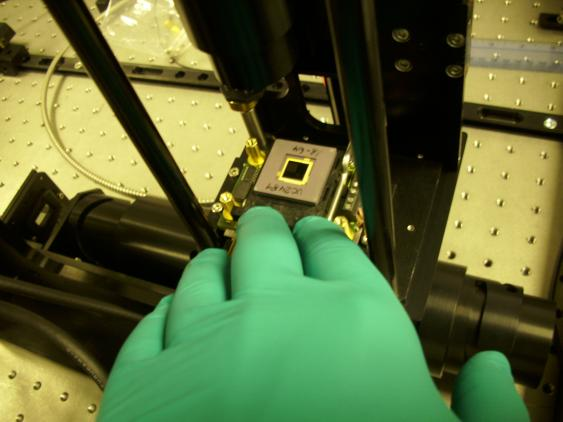
\includegraphics[width=7cm]{mma-plain}
%   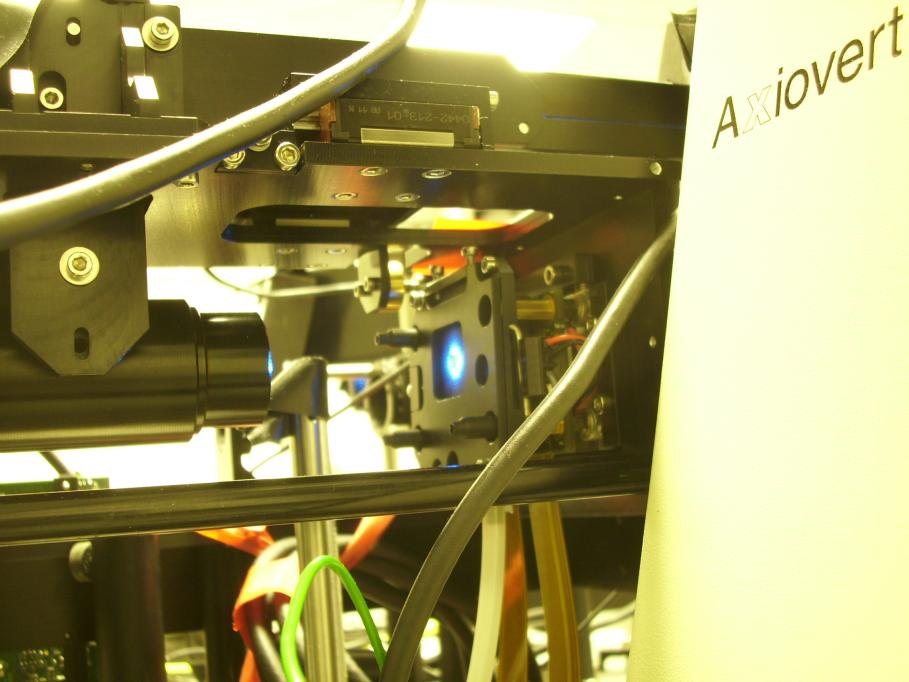
\includegraphics[width=7cm]{mma-ill}
%   \caption{{\bf left:} Micro mirror array chip during installation of
%     the optics. {\bf right:}~Illuminated micro mirror array in the
%     aligned system.}
%   \label{fig:mma-closeup}
% \end{figure}
